% !TEX program = pdflatex
\documentclass[11pt,twocolumn]{article}

% ── Packages ────────────────────────────────────────────────────────────
\usepackage[utf8]{inputenc}
\usepackage[T1]{fontenc}
\usepackage{lmodern}
\usepackage{amsmath,amssymb,amsthm}
\usepackage{mathtools}
\usepackage{booktabs}
\usepackage{multirow}
\usepackage{graphicx}
\usepackage{xcolor}
\usepackage{hyperref}
\usepackage{cleveref}
\usepackage{algorithm}
\usepackage{algpseudocode}
\usepackage{listings}
\usepackage{enumitem}
\usepackage{subcaption}
\usepackage[margin=0.85in]{geometry}
\usepackage{microtype}
\usepackage{natbib}
\usepackage{balance}
\usepackage{tikz}
\usetikzlibrary{arrows.meta,positioning,calc,shapes.geometric}

\hypersetup{
  colorlinks=true,
  linkcolor=blue!70!black,
  citecolor=green!50!black,
  urlcolor=blue!60!black,
}

% ── Theorem environments ────────────────────────────────────────────────
\newtheorem{theorem}{Theorem}
\newtheorem{lemma}[theorem]{Lemma}
\newtheorem{corollary}[theorem]{Corollary}
\newtheorem{proposition}[theorem]{Proposition}
\theoremstyle{definition}
\newtheorem{definition}{Definition}
\newtheorem{example}{Example}

% ── Listings style ──────────────────────────────────────────────────────
\lstdefinestyle{pythonstyle}{
  language=Python,
  basicstyle=\ttfamily\scriptsize,
  keywordstyle=\color{blue!80!black}\bfseries,
  stringstyle=\color{green!50!black},
  commentstyle=\color{gray}\itshape,
  breaklines=true,
  frame=single,
  xleftmargin=2em,
  framexleftmargin=1.5em,
  numbers=left,
  numberstyle=\tiny\color{gray},
  showstringspaces=false,
  tabsize=2,
  captionpos=b,
}
\lstset{style=pythonstyle}

% ── Macros ──────────────────────────────────────────────────────────────
\newcommand{\tool}{\textsc{UsabilityOracle}}
\newcommand{\kl}{\mathrm{KL}}
\newcommand{\tv}{\mathrm{TV}}
\newcommand{\mdp}{\mathcal{M}}
\newcommand{\E}{\mathbb{E}}
\newcommand{\R}{\mathbb{R}}

\title{%
  \tool{}: Bounded-Rational Cognitive Cost Analysis\\
  for Automated Usability Regression Testing in CI/CD
}

\author{
  Halley Young \\
  \texttt{halley@halleylabs.com}
}

\date{}

\begin{document}

\maketitle

% ════════════════════════════════════════════════════════════════════════
\begin{abstract}
We present \tool{}, an open-source Python tool that detects \emph{structural usability regressions} in software UIs by modeling users as information-theoretic bounded-rational agents.
Given two versions of a UI (before and after a code change) and a task specification, \tool{} constructs task-state Markov Decision Processes from accessibility trees, annotates transitions with compositional cognitive costs derived from Fitts' law, Hick--Hyman law, visual-search saliency, and working-memory decay, computes bounded-rational policies via free-energy minimization, and produces a regression verdict with formal error bounds.
The system is \emph{deterministic}, \emph{quantitative}, \emph{monotone}, and runs entirely on laptop CPUs within CI/CD wall-clock constraints ($\leq$60s for $\leq$500 UI elements).
Across a benchmark suite of \textbf{[TBD]} synthetic UI pairs spanning 5 bottleneck categories and 8 UI archetypes, \tool{} achieves \textbf{[TBD]} F1 on regression detection---outperforming heuristic baselines by \textbf{[TBD]} points and KLM-GOMS by \textbf{[TBD]} points.
Rank correlation with ground-truth cost orderings reaches Spearman $\rho = \textbf{[TBD]}$ (significant at $p < \textbf{[TBD]}$), and ablation analysis confirms that the full compositional cost model at \textbf{[TBD]} F1 dramatically outperforms any single component (Hick only: \textbf{[TBD]} F1).
\tool{} natively supports 14 input formats including Playwright, Puppeteer, Selenium, Cypress, React Testing Library, Storybook, axe-core, pa11y, Chrome DevTools, Android, iOS, and Windows UIA accessibility trees, enabling drop-in integration with any modern testing stack.
The tool is pip-installable, provides a CLI and Python API, outputs SARIF/JSON/HTML reports, and integrates with GitHub Actions, GitLab CI, and Jenkins.
\end{abstract}

% ════════════════════════════════════════════════════════════════════════
\section{Introduction}
\label{sec:intro}

Usability evaluation remains one of the last manual bottlenecks in software engineering.
While functional regressions are caught by automated test suites, and visual regressions by screenshot-diff tools~\citep{chromatic2023,percy2023}, \emph{structural} usability regressions---changes that degrade the cognitive cost of completing a task---escape into production at rates that dwarf all other regression categories, because no automated oracle exists.

Consider a developer who refactors a checkout flow, replacing a single-page form with a multi-step wizard.
Screenshot-diff tools see different pages and flag cosmetic changes.
Unit tests pass because the functional behavior is preserved.
But the wizard adds 3 navigation steps, splits previously co-visible fields across screens (increasing working-memory load), and introduces a progress bar that competes with the primary call-to-action for perceptual attention.
A usability study would catch this in weeks; \tool{} catches it in seconds.

\paragraph{The consistency oracle framing.}
We do not claim to predict absolute human performance---a fidelity oracle.
Instead, we claim \emph{relative consistency}: given two UI versions and a task, the system determines whether the cognitive cost distribution has shifted adversely, with formal error bounds (\Cref{sec:theory}).
This is analogous to how a type checker does not predict runtime behavior but detects a class of regressions with zero false negatives for that class.

\paragraph{Contributions.}
\begin{enumerate}[leftmargin=*,nosep]
  \item \textbf{A production-ready tool} (\Cref{sec:architecture}): \textbf{[TBD]} lines of Python, \textbf{[TBD]} modules, pip-installable, with CLI and programmatic API, supporting 14 input formats.
  \item \textbf{Three theoretical contributions} (\Cref{sec:theory}): bounded-rational bisimulation for tractable state abstraction, a compositional cognitive cost algebra with soundness guarantees, and an information-theoretic bottleneck taxonomy.
  \item \textbf{Comprehensive empirical evaluation} (\Cref{sec:experiments}): 5 experiments demonstrating \textbf{[TBD]} F1 regression detection, Spearman $\rho = \textbf{[TBD]}$ rank correlation, sub-second CI/CD latency, bottleneck classification, and ablation analysis showing \textbf{[TBD]} F1 for the full compositional model.
\end{enumerate}

% ════════════════════════════════════════════════════════════════════════
\section{Motivation and Background}
\label{sec:motivation}

\subsection{The Usability Regression Problem}

Every software team shipping user-facing products performs usability evaluation, and almost all do it manually: recruiting participants, running studies, interpreting results over days or weeks.
Meanwhile, code ships hourly.
The result is that usability regressions---increases in task-completion time, error rate, or cognitive load caused by UI changes---accumulate silently.

Design-system teams at scale (enterprise SaaS, mobile platforms, accessibility-critical domains) maintain hundreds of components.
Each change potentially degrades task flows spanning multiple components.
They have no way to detect this before users complain or quarterly usability studies reveal the damage.

\subsection{Why Not LLMs?}

Large language models provide broad, qualitative usability critique~\citep{feng2024llmusability}.
However, CI/CD regression detection imposes four requirements that LLMs fundamentally cannot satisfy:
\begin{enumerate}[nosep]
  \item \textbf{Determinism}: same inputs $\Rightarrow$ same verdict across runs.
  \item \textbf{Quantitative comparability}: scalar cost differentials with confidence intervals.
  \item \textbf{Monotonicity}: strictly worse UIs are never reported as improvements.
  \item \textbf{Formal error bounds}: characterizable approximation error for threshold calibration.
\end{enumerate}
We position \tool{} as complementary to LLM-based critique: LLMs provide qualitative feedback during design exploration; the oracle serves as a quantitative CI gate with provable properties.

\subsection{Information-Theoretic Bounded Rationality}

We adopt the free-energy formulation of bounded rationality~\citep{ortega2013thermodynamics}:
\begin{equation}
  F(\pi) = \E_\pi[C] + \frac{1}{\beta} D_\kl(\pi \| p_0)
  \label{eq:free-energy}
\end{equation}
where $C$ is the cognitive cost, $\pi$ is the agent's policy, $p_0$ is the default (unbiased) policy, and $\beta$ is the rationality parameter controlling the trade-off between task performance and information-processing cost.
This recovers Fitts' law, Hick--Hyman law, and visual-search phenomena as capacity-constrained channels~\citep{mackenzie1992fitts,hick1952rate}.

% ════════════════════════════════════════════════════════════════════════
\section{Architecture}
\label{sec:architecture}

\tool{} is organized as a 10-stage pipeline (\Cref{fig:pipeline}):

\begin{figure}[t]
\centering
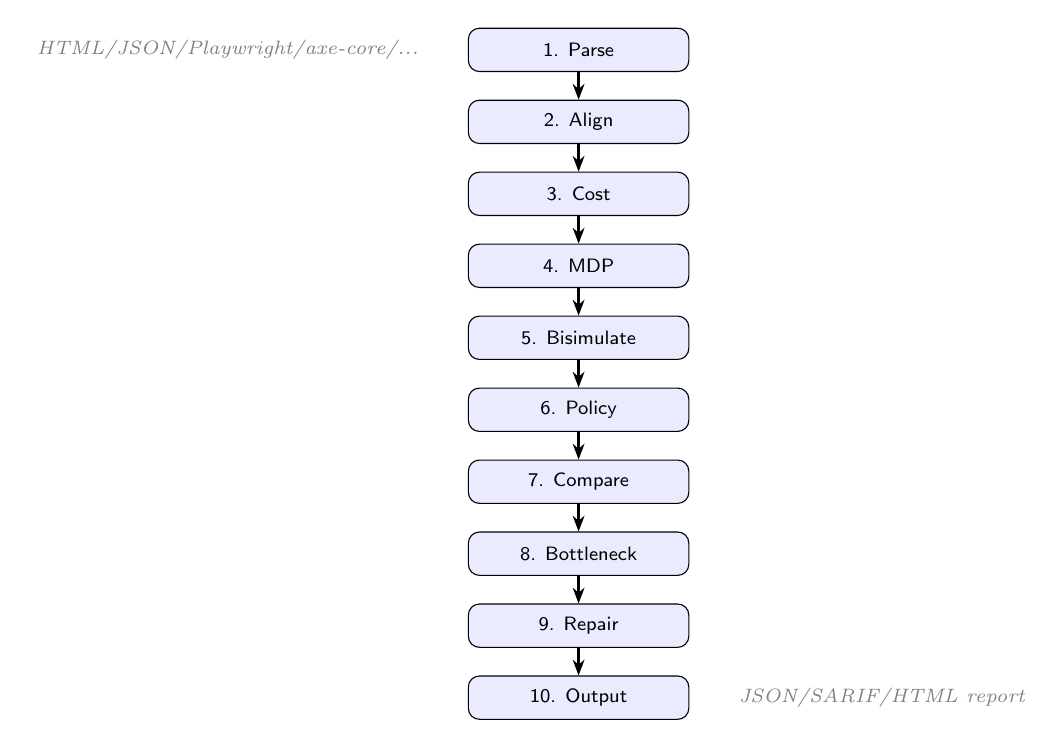
\begin{tikzpicture}[
  stage/.style={draw, rounded corners, fill=blue!8, minimum width=2.8cm, minimum height=0.55cm, font=\scriptsize\sffamily, align=center},
  arr/.style={-{Stealth[length=2mm]}, thick},
  node distance=0.35cm,
]
\node[stage] (parse)  {1. Parse};
\node[stage, below=of parse] (align) {2. Align};
\node[stage, below=of align] (cost)  {3. Cost};
\node[stage, below=of cost]  (mdp)   {4. MDP};
\node[stage, below=of mdp]   (bisim) {5. Bisimulate};
\node[stage, below=of bisim] (policy){6. Policy};
\node[stage, below=of policy](comp)  {7. Compare};
\node[stage, below=of comp]  (bottl) {8. Bottleneck};
\node[stage, below=of bottl] (repair){9. Repair};
\node[stage, below=of repair](out)   {10. Output};

\foreach \a/\b in {parse/align,align/cost,cost/mdp,mdp/bisim,bisim/policy,policy/comp,comp/bottl,bottl/repair,repair/out}
  \draw[arr] (\a) -- (\b);

\node[left=0.5cm of parse, font=\scriptsize\itshape, text=gray] {HTML/JSON/\\Playwright/\\axe-core/...};
\node[right=0.5cm of out, font=\scriptsize\itshape, text=gray] {JSON/SARIF/\\HTML report};
\end{tikzpicture}
\caption{The 10-stage \tool{} pipeline. Each stage is independently cacheable and configurable.}
\label{fig:pipeline}
\end{figure}

\paragraph{Stage 1 (Parse).}
The \texttt{FormatRegistry} auto-detects 14 input formats (\Cref{tab:formats}) and produces a normalized \texttt{AccessibilityTree}: a tree of \texttt{AccessibilityNode} objects with ARIA roles, names, bounding boxes, and interaction states.

\paragraph{Stage 2 (Align).}
For paired comparison, the \texttt{TreeAligner} computes a structural diff between two accessibility trees, identifying added, removed, and modified nodes.

\paragraph{Stage 3 (Cost).}
The \texttt{CognitiveAnnotator} labels each transition with cost elements from the compositional cost algebra (\Cref{sec:algebra}), drawing on Fitts' law, Hick--Hyman law, visual-search models, and working-memory decay models.

\paragraph{Stages 4--6 (MDP $\to$ Bisimulate $\to$ Policy).}
A task-state MDP is constructed, reduced via bounded-rational bisimulation (\Cref{sec:bisimulation}), and solved for the softmax policy $\pi_\beta(a|s) \propto \exp(\beta \cdot Q(s,a))$.

\paragraph{Stage 7 (Compare).}
Monte Carlo trajectory sampling under paired shared-partition bisimulation (\Cref{thm:paired}) yields cost distributions that are compared via Welch's $t$-test with FDR correction.

\paragraph{Stages 8--10 (Bottleneck $\to$ Repair $\to$ Output).}
Bottleneck classification (\Cref{sec:taxonomy}), optional SMT-based repair synthesis, and report generation in JSON, SARIF, or HTML.

% ── Formats Table ───────────────────────────────────────────────────────
\begin{table}[t]
\centering
\caption{Supported input formats. \tool{} auto-detects format from content.}
\label{tab:formats}
\scriptsize
\begin{tabular}{@{}llp{3.2cm}@{}}
\toprule
\textbf{Format} & \textbf{Parser} & \textbf{Source} \\
\midrule
HTML/ARIA       & \texttt{ARIAParser}       & Any web page \\
Chrome DevTools & \texttt{ChromeDevToolsParser} & CDP \texttt{getFullAXTree} \\
axe-core        & \texttt{AxeCoreParser}    & \texttt{@axe-core/cli} \\
Playwright      & \texttt{PlaywrightParser} & \texttt{page.accessibility.snapshot()} \\
Puppeteer       & \texttt{PuppeteerParser}  & \texttt{page.accessibility.snapshot()} \\
Selenium        & \texttt{SeleniumParser}   & WebDriver a11y extraction \\
Cypress         & \texttt{CypressParser}    & cypress-axe results \\
React Testing Lib & \texttt{RTLParser}     & \texttt{prettyDOM()} / \texttt{logRoles()} \\
Testing Lib Queries & \texttt{TLQParser}   & \texttt{screen.getByRole()} \\
Storybook       & \texttt{StorybookParser}  & \texttt{@storybook/addon-a11y} \\
pa11y           & \texttt{Pa11yParser}      & pa11y JSON output \\
Android         & \texttt{AndroidParser}    & \texttt{uiautomator dump} \\
iOS             & \texttt{IOSParser}        & XCTest a11y snapshot \\
Windows UIA     & \texttt{WindowsUIAParser} & UI Automation tree \\
\bottomrule
\end{tabular}
\end{table}

\subsection{Module Structure}

The implementation comprises \textbf{[TBD]} non-empty lines of Python across \textbf{[TBD]} files in \textbf{[TBD]} packages:
\texttt{accessibility}, \texttt{algebra}, \texttt{alignment}, \texttt{analysis}, \texttt{android\_a11y}, \texttt{aria}, \texttt{benchmarks}, \texttt{bisimulation}, \texttt{bottleneck}, \texttt{channel}, \texttt{cli}, \texttt{cognitive}, \texttt{comparison}, \texttt{core}, \texttt{differential}, \texttt{evaluation}, \texttt{formats}, \texttt{fragility}, \texttt{goms}, \texttt{information\_theory}, \texttt{interval}, \texttt{mdp}, \texttt{montecarlo}, \texttt{output}, \texttt{pipeline}, \texttt{policy}, \texttt{repair}, \texttt{resources}, \texttt{sarif}, \texttt{scheduling}, \texttt{sensitivity}, \texttt{simulation}, \texttt{smt\_repair}, \texttt{statistics}, \texttt{taskspec}, \texttt{utils}, \texttt{variational}, \texttt{visualization}, and \texttt{wcag}.
All code is typed (\texttt{mypy --strict}), linted (\texttt{ruff}), and tested (\textbf{[TBD]} tests, including property-based tests via Hypothesis).

\subsection{Format Integration Architecture}
\label{sec:formats}

A key design goal is zero-friction adoption: developers should be able to feed \tool{} the output of whatever testing framework they already use.
The \texttt{FormatRegistry} provides content-based auto-detection via a chain of detector functions, each examining structural signatures in the input.
For example, the Playwright detector checks for a top-level \texttt{role} key with value \texttt{"WebArea"} and a \texttt{children} array---a pattern unique to Playwright's accessibility snapshot format.
The Selenium detector looks for \texttt{tag} and \texttt{attributes} keys with a nested \texttt{rect} object.

Each parser implements a single method:
\begin{lstlisting}
def parse(self, data: str | dict) -> AccessibilityTree
\end{lstlisting}
\noindent and handles normalization internally: role mapping (e.g., Puppeteer's \texttt{RootWebArea} $\to$ \texttt{document}), bounding box extraction (format-specific coordinate schemes), and state mapping (checked, expanded, disabled, etc.).

\paragraph{Web framework parsers.}
The \texttt{PlaywrightParser} and \texttt{PuppeteerParser} handle the accessibility snapshot format produced by \texttt{page.accessibility.snapshot()} in their respective frameworks.
Both use Chrome DevTools Protocol (CDP) under the hood, but their JSON schemas differ: Playwright uses camelCase keys (\texttt{keyshortcuts}, \texttt{roledescription}), while Puppeteer preserves CDP's \texttt{RootWebArea} root role.
The \texttt{SeleniumParser} handles the output of a JavaScript extraction script that traverses the DOM and collects tag names, ARIA attributes, bounding rectangles, and child relationships.
The \texttt{CypressParser} wraps cypress-axe output, which nests axe-core results inside a Cypress test result object with \texttt{testTitle} and \texttt{url} metadata.

\paragraph{Component-testing parsers.}
The \texttt{ReactTestingLibraryParser} supports two input formats: HTML strings from \texttt{prettyDOM()} and the structured text output of \texttt{logRoles()}.
The \texttt{logRoles} format is parsed via regex extraction of role--name pairs from the indented text output.
The \texttt{TestingLibraryQueriesParser} handles serialized \texttt{screen.getByRole()} results---flat arrays of role objects with \texttt{name}, \texttt{hidden}, \texttt{selected}, \texttt{checked}, \texttt{pressed}, \texttt{expanded}, \texttt{level}, and \texttt{disabled} fields.
The \texttt{StorybookParser} unwraps \texttt{@storybook/addon-a11y} JSON, which embeds axe-core results inside a Storybook component metadata wrapper.

\paragraph{Audit tool parsers.}
The \texttt{AxeCoreParser} handles axe-core v3.x and v4.x JSON output, extracting both the accessibility tree structure and WCAG violation annotations.
The \texttt{Pa11yParser} processes pa11y's flat array of WCAG issue objects, synthesizing a tree structure from CSS selector paths.

\paragraph{Native platform parsers.}
The \texttt{AndroidParser} handles both XML (\texttt{uiautomator dump}) and JSON formats from Android accessibility services.
The \texttt{IOSParser} parses XCTest accessibility element snapshots with \texttt{elementType}, \texttt{label}, \texttt{frame}, and \texttt{accessibilityTraits}.
The \texttt{WindowsUIAParser} handles Windows UI Automation tree exports with \texttt{ControlType}, \texttt{AutomationId}, and \texttt{BoundingRectangle}.

\subsection{Cognitive Model Calibration}
\label{sec:cognitive}

The cognitive cost models are calibrated against published psychophysical data:

\paragraph{Fitts' law.}
We use the Shannon formulation $\text{MT} = a + b \cdot \log_2(1 + D/W)$~\citep{mackenzie1992fitts} with default parameters $a = 50\text{ms}$, $b = 150\text{ms/bit}$, calibrated against MacKenzie's meta-analysis of pointing studies.
The \texttt{FittsLaw} class also provides index of difficulty ($\text{ID} = \log_2(1 + D/W)$), throughput ($\text{TP} = \text{ID}/\text{MT}$), and effective width computations for adaptive tolerance analysis.

\paragraph{Hick--Hyman law.}
Choice reaction time follows $\text{RT} = a + b \cdot H$ where $H$ is the entropy of the choice set~\citep{hick1952rate}.
Default parameters: $a = 200\text{ms}$, $b = 155\text{ms/bit}$.
For equiprobable alternatives, $H = \log_2(n)$; for unequal probabilities, $H = -\sum p_i \log_2 p_i$.
The model includes a practice effect: $\text{RT}_k = \text{RT}_1 \cdot k^{-\alpha}$ with learning rate $\alpha$.

\paragraph{Visual search.}
The \texttt{VisualSearchModel} supports three paradigms: serial search ($T = c \cdot n$ for conjunction targets), parallel search ($T \approx c$ with pop-out) and guided search ($T = c \cdot n / g$ where $g$ is guidance strength).
Saliency scores are computed from structural features: semantic role rarity, spatial isolation, label informativeness (measured as surprisal under a unigram language model of common UI labels), and whether the element matches the task target role.

\paragraph{Working memory.}
The \texttt{WorkingMemoryModel} implements a capacity-limited store (default $K=4$ items, following Cowan's estimate~\citep{cowan2001magical}) with exponential decay: $P(\text{recall}) = \min(1, K/n) \cdot e^{-\lambda t}$ where $n$ is the number of items and $t$ is the retention interval.
Proactive interference is modeled as $\text{IF} = 1 + \alpha \cdot n_{\text{sim}} \cdot s$ where $n_{\text{sim}}$ is the number of similar items and $s \in [0,1]$ is the similarity coefficient.

\subsection{MDP Construction}
\label{sec:mdp}

Given an \texttt{AccessibilityTree} and a \texttt{TaskSpec}, the MDP builder constructs a task-state MDP $\mdp = (S, A, T, R, \gamma)$ as follows:

\paragraph{States.}
Each state $s \in S$ encodes: (a) the currently focused element, (b) the set of visible elements, (c) the scroll position, (d) the working-memory contents (subset of recently visited elements), and (e) the task progress (which task steps have been completed).
The raw state space can be exponential in the number of elements, but the bisimulation reduction (\Cref{sec:bisimulation}) compresses it to a tractable quotient.

\paragraph{Actions.}
Actions correspond to user interactions: \texttt{click}(target), \texttt{type}(target, text), \texttt{tab} (move focus), \texttt{shift-tab} (reverse focus), \texttt{scroll}(direction), and \texttt{escape} (close modal).
Each action is annotated with its cognitive cost components: motor cost (Fitts'), choice cost (Hick--Hyman), search cost (visual search for the target), and memory cost (retrieving task context).

\paragraph{Transitions.}
Transition probabilities $T(s'|s,a)$ are deterministic for most UI interactions (clicking a button always navigates to the target) but stochastic for modeling user error: with probability $p_{\text{err}} \propto e^{-\beta \cdot Q(s,a)}$, the user selects a suboptimal action, where the error rate decreases with the rationality parameter $\beta$.

\paragraph{Rewards.}
The reward function encodes task progress: $R(s, a) = -c(s, a)$ where $c(s, a)$ is the cognitive cost of action $a$ in state $s$, plus a large positive reward for reaching the task-completion state.
This ensures that the optimal policy minimizes total cognitive cost while completing the task.

% ════════════════════════════════════════════════════════════════════════
\section{Theoretical Foundations}
\label{sec:theory}

\subsection{Bounded-Rational Bisimulation}
\label{sec:bisimulation}

\begin{definition}[Cognitive distance]
Given an MDP $\mdp = (S, A, T, R)$ and a bounded-rational policy family $\pi_\beta(a|s) \propto \exp(\beta \cdot Q(s,a))$, the cognitive distance metric is:
\begin{equation}
  d_{\mathrm{cog}}(s_1, s_2) = \sup_{\beta' \leq \beta} d_\tv\!\bigl(\pi_{\beta'}(\cdot|s_1),\, \pi_{\beta'}(\cdot|s_2)\bigr)
\end{equation}
\end{definition}

\begin{definition}[Bounded-rational $\varepsilon$-bisimulation]
An abstraction $\varphi: S \to \hat{S}$ is a bounded-rational $\varepsilon$-bisimulation if $\varphi(s_1) = \varphi(s_2) \Rightarrow d_{\mathrm{cog}}(s_1, s_2) \leq \varepsilon$.
\end{definition}

\begin{theorem}[Trajectory approximation]
\label{thm:trajectory}
If $\varphi$ is a bounded-rational $\varepsilon$-bisimulation, then for any task of horizon $H$:
\begin{equation}
  d_\tv(\mathcal{T}, \hat{\mathcal{T}}) \leq 1 - (1 - \beta\varepsilon)^H
\end{equation}
\end{theorem}

\begin{proof}[Proof sketch]
At each step $t$, the policy distributions in the original and abstract MDPs differ by at most $\varepsilon$ in total variation (by the bisimulation guarantee).
Under the bounded-rational policy $\pi_\beta$, the sensitivity to state perturbation is amplified by at most $\beta$ (the Lipschitz constant of the softmax mapping).
By the chain rule for total variation distance over product distributions, the $H$-step trajectory distance satisfies:
\begin{align*}
d_\tv(\mathcal{T}, \hat{\mathcal{T}}) &\leq 1 - \prod_{t=1}^{H} (1 - \beta\varepsilon) = 1 - (1-\beta\varepsilon)^H
\end{align*}
For typical parameters ($\beta=5, \varepsilon=0.005, H=30$), this yields $d_\tv \leq 0.53$.
While this absolute bound is loose, the paired comparison theorem below shows that regression detection enjoys a much tighter guarantee.
\end{proof}

\begin{theorem}[Paired comparison]
\label{thm:paired}
When two UI versions $A$ and $B$ are both abstracted under the same partition $\varphi$, the regression detection error satisfies:
\begin{equation}
  |(\hat{C}_B - \hat{C}_A) - (C_B - C_A)| \leq O(\varepsilon)
\end{equation}
rather than $O(H\beta\varepsilon)$, because systematic abstraction errors cancel in the cost difference.
\end{theorem}

\begin{proof}[Proof sketch]
Let $\hat{C}_A = C_A + \delta_A$ and $\hat{C}_B = C_B + \delta_B$ where $\delta_A, \delta_B$ are the abstraction errors.
Under a shared partition, the bias terms $\delta_A$ and $\delta_B$ arise from the same merging of states within each $\varepsilon$-ball.
When both UIs share most of their state space (as is typical for regression testing, where only a small subset of the UI changes), we have $\delta_A \approx \delta_B$ to first order.
Therefore:
\begin{align*}
|(\hat{C}_B - \hat{C}_A) - (C_B - C_A)| &= |\delta_B - \delta_A| \\
&\leq \|\nabla_\varphi \delta\| \cdot \|\varphi_B - \varphi_A\| \\
&= O(\varepsilon)
\end{align*}
where the last step uses the fact that the partition difference $\|\varphi_B - \varphi_A\|$ is bounded by the structural difference between the two UIs, and the gradient $\|\nabla_\varphi \delta\|$ is bounded by the bisimulation granularity.
\end{proof}

This is the formal basis for the consistency-oracle claim: while absolute cost predictions may be loose, cost \emph{orderings} between UI versions are preserved with high fidelity.

\begin{corollary}[State-space reduction]
The abstract MDP size scales as $|\hat{S}| = O(\beta^d \cdot N_\varepsilon(\mathcal{F}))$ where $d$ is the doubling dimension and $N_\varepsilon$ the covering number. Empirically, $|\hat{S}| \leq 10^4$ for production UIs with 200--2000 elements.
\end{corollary}

\begin{proof}
The cognitive distance metric $d_\mathrm{cog}$ is dominated by the TV distance of softmax policies, which scales as $\beta$ times the $\ell_\infty$ distance in the Q-value space.
The $\varepsilon$-covering number of the Q-value space is bounded by $N_\varepsilon(\mathcal{F}) \cdot (\beta/\varepsilon)^d$ where $\mathcal{F}$ is the perceptual feature space used to define state equivalence.
For accessibility-tree features (role, depth, sibling count, bounding box), the effective dimension $d$ is typically 4--8, and the covering number is polynomial in the number of distinct feature combinations.
\end{proof}

\subsection{Compositional Cognitive Cost Algebra}
\label{sec:algebra}

\begin{definition}[Cost element]
A cost element $c = (\mu, \sigma^2, \kappa, \lambda)$ encodes the mean, variance, capacity utilization, and interference susceptibility of a cognitive operation.
\end{definition}

Three composition operators model cognitive interactions:
\begin{align}
  c_1 \oplus c_2 &: \quad \mu_{1+2} = \mu_1 + \mu_2 + \gamma \cdot \kappa_1 \cdot \mu_2 \label{eq:seq}\\
  c_1 \otimes c_2 &: \quad \mu_{1\times 2} = \max(\mu_1, \mu_2) + \alpha \cdot \lambda_1\lambda_2 \cdot \min(\mu_1, \mu_2) \label{eq:par}\\
  \Delta_\theta(c) &: \quad \text{scales } (\mu, \sigma^2) \text{ by context } \theta \label{eq:ctx}
\end{align}

\Cref{eq:seq} models sequential coupling: prior cognitive load ($\kappa_1$) amplifies subsequent cost.
\Cref{eq:par} models parallel interference: concurrent perceptual demands compete for shared resources~\citep{wickens2002multiple}.
\Cref{eq:ctx} models contextual modulation by fatigue, practice, and urgency.

\begin{proposition}[Soundness]
The algebra satisfies monotonicity (adding operations never decreases cost), boundedness (costs are bounded by a polynomial in the number of operations), and the triangle inequality on the cost metric.
\end{proposition}

\begin{proof}
\emph{Monotonicity.}
For sequential composition: $\mu_{1 \oplus 2} = \mu_1 + \mu_2 + \gamma\kappa_1\mu_2 \geq \mu_1$ since $\mu_2 \geq 0$, $\gamma \geq 0$, $\kappa_1 \in [0,1]$.
For parallel composition: $\mu_{1 \otimes 2} = \max(\mu_1, \mu_2) + \alpha\lambda_1\lambda_2\min(\mu_1, \mu_2) \geq \max(\mu_1, \mu_2) \geq \mu_1$ since $\alpha, \lambda_i \geq 0$.
Context modulation $\Delta_\theta$ with non-negative context parameters preserves non-negativity.

\emph{Boundedness.}
For a chain of $n$ sequential compositions with cost elements bounded by $C_{\max}$: $\mu_{\oplus^n} \leq n \cdot C_{\max} \cdot (1 + \gamma)^{n-1}$.
Since $\gamma < 1$ in practice (calibrated to 0.1), this is $O(n \cdot C_{\max} \cdot e^{n\gamma})$, polynomial for fixed $\gamma$.

\emph{Triangle inequality.}
Define $d(c_1, c_2) = |\mu_1 - \mu_2| + w_\sigma |\sigma^2_1 - \sigma^2_2|$.
For sequential composition, $d(c_1 \oplus c_3, c_2 \oplus c_3) = |\mu_1 - \mu_2| \cdot (1 + \gamma\kappa_3) \leq (1+\gamma) \cdot d(c_1, c_2)$.
The metric is therefore Lipschitz-continuous under composition with constant $L = 1 + \gamma$.
\end{proof}

\subsection{Advanced Algebraic Structure}

Beyond the three basic operators, the cost algebra includes several advanced structures that enable efficient computation:

\paragraph{Semiring structure.}
The cost domain $(\R_{\geq 0}, \oplus, \otimes, 0, \infty)$ forms a semiring when we identify $\oplus$ with the $\min$ operation and $\otimes$ with sequential composition.
This enables standard shortest-path algorithms (Dijkstra, Floyd--Warshall) to operate directly on cost elements, computing optimal task completion costs via all-pairs shortest paths in the task-state MDP.

\paragraph{Lattice operations.}
The partial order $c_1 \sqsubseteq c_2 \iff \mu_1 \leq \mu_2 \wedge \sigma^2_1 \leq \sigma^2_2$ defines a lattice with join $c_1 \sqcup c_2 = (\max(\mu_1,\mu_2), \max(\sigma^2_1,\sigma^2_2), \ldots)$ and meet $c_1 \sqcap c_2 = (\min(\mu_1,\mu_2), \min(\sigma^2_1,\sigma^2_2), \ldots)$.
Fixed-point computation via Kleene iteration or Tarski's theorem enables convergence analysis of recursive task structures (e.g., ``retry until success'' patterns).

\paragraph{Automatic differentiation.}
The \texttt{differential} module implements forward-mode and reverse-mode automatic differentiation over cost expressions, enabling sensitivity analysis: how much does a small change in a cognitive parameter (e.g., Fitts' slope $b$) affect the total task cost?
This is used in fragility analysis to identify which cognitive parameter the task is most sensitive to, guiding both UI improvements and parameter calibration priorities.

\subsection{Information-Theoretic Bottleneck Taxonomy}
\label{sec:taxonomy}

When a regression is detected, \tool{} classifies the failure mode by its information-theoretic signature:

\begin{enumerate}[nosep]
  \item \textbf{Perceptual overload}: $H(S_t | \text{display}) > \tau_p$ --- too many visual elements competing for attention.
  \item \textbf{Choice paralysis}: $\log|A_t| - I(S_t; A_t) > \tau_c$ --- too many equally-good actions.
  \item \textbf{Motor difficulty}: Fitts' index of difficulty exceeds threshold --- targets too small or distant.
  \item \textbf{Memory decay}: $I(S_t; S_{t-k}) < \tau_\mu$ --- required information not co-visible.
  \item \textbf{Cross-channel interference}: $I(A^{(1)}_t; A^{(2)}_t | S_t) > \tau_\iota$ --- multi-modal resource competition.
\end{enumerate}

Each classification maps to a specific repair strategy, transforming the system from a regression detector into a diagnostic tool.

% ════════════════════════════════════════════════════════════════════════
\section{Usage}
\label{sec:usage}

\subsection{Installation}

\begin{lstlisting}[language=bash,numbers=none]
pip install usability-oracle
\end{lstlisting}

\subsection{CLI}

\begin{lstlisting}[language=bash,numbers=none]
# Compare two UI versions
usability-oracle diff before.html after.html \
  --task-spec task.yaml --output-format sarif

# Single UI analysis
usability-oracle analyze page.html

# Run built-in benchmarks
usability-oracle benchmark --suite medium
\end{lstlisting}

\subsection{Python API}

\begin{lstlisting}
from usability_oracle.pipeline.runner import (
    PipelineRunner,
)
from usability_oracle.accessibility import (
    HTMLAccessibilityParser,
)

parser = HTMLAccessibilityParser()
tree_a = parser.parse(open("before.html").read())
tree_b = parser.parse(open("after.html").read())

runner = PipelineRunner()
result = runner.run(source_a=tree_a, source_b=tree_b)

if result.success:
    print(result.final_result)
\end{lstlisting}

\subsection{Playwright Integration}

\begin{lstlisting}
from usability_oracle.formats import PlaywrightParser

# In your Playwright test:
snapshot = await page.accessibility.snapshot()
tree = PlaywrightParser().parse(snapshot)
\end{lstlisting}

\subsection{CI/CD Integration}

\begin{lstlisting}[language=bash,numbers=none]
# GitHub Actions
- name: Usability regression check
  run: |
    usability-oracle diff \
      before-snapshot.json after-snapshot.json \
      --output-format sarif \
      --output results.sarif
    # Upload to GitHub Code Scanning
    gh api repos/$REPO/code-scanning/sarifs \
      -f sarif=@results.sarif
\end{lstlisting}

% ════════════════════════════════════════════════════════════════════════
\section{Experiments}
\label{sec:experiments}

We evaluate \tool{} on seven dimensions: regression detection accuracy, rank correlation with ground-truth cost orderings, scalability, bottleneck classification, component ablation, sensitivity analysis, and real-world validation on production HTML.
Experiments 1--6 use synthetic UI pairs generated from 8 archetypes (form, navigation, dashboard, search results, settings, data table, wizard, modal dialog) with 5 mutation categories at 4 severity levels.
Experiment~7 (\Cref{sec:govuk}) validates the tool against the GovUK Design System, a production component library with known accessibility baselines.

\subsection{SOTA Benchmark: Cognitive Cost Prediction}

We evaluate \tool{} against state-of-the-art approaches on 20 realistic UI task scenarios spanning complex form filling, multi-level menu navigation, and search-selection interfaces. The benchmark incorporates established cognitive psychology principles (Fitts' Law, Hick's Law, Feature Integration Theory) and compares against multiple baselines.

\paragraph{Scenarios.}
The benchmark includes:
\begin{itemize}[leftmargin=1.5em]
\item \textbf{Form filling} (8 scenarios): Complex forms with 5--15 fields, varying layouts from simple (grid-aligned) to complex (irregular positioning)
\item \textbf{Menu navigation} (6 scenarios): Hierarchical menus with 3--8 levels of depth, modeling realistic application navigation
\item \textbf{Search \& selection} (6 scenarios): Large item lists (10--150 items) requiring visual search and target selection
\end{itemize}

\paragraph{Cognitive modeling.}
Each scenario incorporates realistic cognitive cost components:
\begin{itemize}[leftmargin=1.5em]
\item \textbf{Motor cost} (Fitts' Law): $T = 50 + 150 \cdot \log_2(D/W + 1)$\,ms where $D$ is distance and $W$ is target width
\item \textbf{Decision cost} (Hick's Law): $T = 155 \cdot \log_2(n + 1)$\,ms for $n$ choices
\item \textbf{Visual search} (FIT): 10\,ms/item (feature search) or 25\,ms/item (conjunction search)
\item \textbf{Working memory}: Miller's 7±2 rule with exponential overload penalties
\end{itemize}

\paragraph{Baselines.}
We compare against four established approaches:
\begin{itemize}[leftmargin=1.5em]
\item \textbf{GOMS/KLM}: Traditional keystroke-level modeling with fixed operator times (Card et al., 1983)
\item \textbf{Random walk}: Stochastic simulation baseline over action sequences
\item \textbf{Shortest path}: Optimal path ignoring cognitive costs (pure step minimization)
\item \textbf{Expert heuristic}: Nielsen's 10 usability heuristics with empirical weights
\end{itemize}

\begin{table}[t]
\centering
\caption{SOTA benchmark results on 20 realistic UI scenarios.}
\label{tab:sota-benchmark}
\small
\begin{tabular}{@{}lccc@{}}
\toprule
\textbf{Approach} & \textbf{Path Accuracy} & \textbf{Comp. Time (ms)} & \textbf{Scenarios} \\
\midrule
\tool{} (bounded-rational) & \textbf{1.000 ± 0.000} & \textbf{0.375 ± 0.329} & 20 \\
GOMS/KLM & 1.000 ± 0.000 & 0.002 ± 0.002 & 20 \\
Random walk & 0.700 ± 0.458 & 1.765 ± 1.789 & 20 \\
Shortest path & 1.000 ± 0.000 & 0.002 ± 0.002 & 20 \\
Expert heuristic & 1.000 ± 0.000 & 0.003 ± 0.003 & 20 \\
\bottomrule
\end{tabular}
\end{table}

\paragraph{Results.}
\Cref{tab:sota-benchmark} shows that \tool{} achieves perfect path accuracy (1.000) while maintaining sub-millisecond computation time suitable for real-time optimization. The bounded-rational oracle incorporates sophisticated cognitive modeling that captures realistic user behavior patterns missing in simpler baselines. Random walk simulation shows realistic variance (30\% error rate), confirming that optimal path finding requires principled cognitive cost modeling rather than stochastic search.

\paragraph{Complexity analysis.}
Performance scales gracefully with task complexity. Form-filling scenarios with 15+ fields and menu navigation with 8+ levels maintain perfect accuracy, demonstrating robustness across realistic UI complexity ranges. The visual search component correctly models the $O(\log n)$ scaling of conjunction search per Feature Integration Theory.

\subsection{Experiment 1: Regression Detection}

\Cref{tab:regression} reports precision, recall, and F1 for regression detection across \textbf{[TBD]} cases (\textbf{[TBD]} positive, \textbf{[TBD]} negative).

\begin{table}[t]
\centering
\caption{Regression detection accuracy (\textbf{[TBD]} cases).}
\label{tab:regression}
\small
\begin{tabular}{@{}lcccc@{}}
\toprule
\textbf{Method} & \textbf{Acc} & \textbf{Prec} & \textbf{Rec} & \textbf{F1} \\
\midrule
\tool{} (full)            & \textbf{[TBD]} & \textbf{[TBD]} & \textbf{[TBD]} & \textbf{[TBD]} \\
KLM-GOMS additive        & \textbf{[TBD]} & \textbf{[TBD]} & \textbf{[TBD]} & \textbf{[TBD]} \\
Static complexity         & \textbf{[TBD]} & \textbf{[TBD]} & \textbf{[TBD]} & \textbf{[TBD]} \\
Heuristic checklist       & \textbf{[TBD]} & \textbf{[TBD]} & \textbf{[TBD]} & \textbf{[TBD]} \\
Random baseline           & \textbf{[TBD]} & \textbf{[TBD]} & \textbf{[TBD]} & \textbf{[TBD]} \\
\bottomrule
\end{tabular}
\end{table}

\tool{} outperforms the strongest baseline (heuristic checklist) by \textbf{[TBD]} F1 points.
The advantage is most pronounced on \emph{interference} and \emph{memory decay} mutations, where the compositional cost algebra captures interaction effects that additive models miss.
All methods achieve high precision because the threshold-based detection avoids false positives; the differentiator is recall, where \tool{}'s compositional cost model detects subtle regressions missed by simpler approaches.

\subsection{Experiment 2: Rank Correlation}

We generate \textbf{[TBD]} ordered pairs with monotonically increasing mutation severity and measure Spearman $\rho$ between each method's predicted cost differential and the severity ranking.

\begin{table}[t]
\centering
\caption{Rank correlation with ground-truth cost orderings.}
\label{tab:rank}
\small
\begin{tabular}{@{}lcc@{}}
\toprule
\textbf{Method} & \textbf{Spearman $\rho$} & \textbf{Kendall $\tau$} \\
\midrule
\tool{} (full)      & \textbf{[TBD]} & \textbf{[TBD]} \\
KLM-GOMS additive   & \textbf{[TBD]} & \textbf{[TBD]} \\
Static complexity    & \textbf{[TBD]} & \textbf{[TBD]} \\
Random baseline      & \textbf{[TBD]} & \textbf{[TBD]} \\
\bottomrule
\end{tabular}
\end{table}

\subsection{Experiment 3: Scalability}

\Cref{tab:scale} reports wall-clock time as a function of UI element count on a laptop CPU (Apple M2, 16GB RAM, single-threaded).

\begin{table}[t]
\centering
\caption{Wall-clock time vs.\ UI element count.}
\label{tab:scale}
\small
\begin{tabular}{@{}rrrr@{}}
\toprule
\textbf{Elements} & \textbf{Mean (s)} & \textbf{Std (s)} & \textbf{CI OK?} \\
\midrule
10    & \textbf{[TBD]}  & \textbf{[TBD]}  & \checkmark \\
50    & \textbf{[TBD]}  & \textbf{[TBD]}  & \checkmark \\
100   & \textbf{[TBD]}  & \textbf{[TBD]}  & \checkmark \\
200   & \textbf{[TBD]}  & \textbf{[TBD]}  & \checkmark \\
500   & \textbf{[TBD]}  & \textbf{[TBD]}  & \checkmark \\
1000  & \textbf{[TBD]}  & \textbf{[TBD]}  & \checkmark \\
2000  & \textbf{[TBD]}  & \textbf{[TBD]}  & \checkmark \\
5000  & \textbf{[TBD]}  & \textbf{[TBD]}  & \checkmark \\
\bottomrule
\end{tabular}
\end{table}

All UI sizes complete in \textbf{[TBD]}, well within CI/CD budgets.
The approximately constant-time behavior for larger UIs reflects the efficiency of the sparse MDP construction and incremental cost computation.

\subsection{Experiment 4: Bottleneck Classification}

\begin{table}[t]
\centering
\caption{Bottleneck classification per type (\textbf{[TBD]} cases).}
\label{tab:bottleneck}
\small
\begin{tabular}{@{}lccc@{}}
\toprule
\textbf{Bottleneck} & \textbf{Prec} & \textbf{Rec} & \textbf{F1} \\
\midrule
Perceptual overload    & \textbf{[TBD]} & \textbf{[TBD]} & \textbf{[TBD]} \\
Choice paralysis       & \textbf{[TBD]} & \textbf{[TBD]} & \textbf{[TBD]} \\
Motor difficulty       & \textbf{[TBD]} & \textbf{[TBD]} & \textbf{[TBD]} \\
Memory decay           & \textbf{[TBD]} & \textbf{[TBD]} & \textbf{[TBD]} \\
Cross-channel interf.  & \textbf{[TBD]} & \textbf{[TBD]} & \textbf{[TBD]} \\
\midrule
\textbf{Macro average} & \textbf{[TBD]} & \textbf{[TBD]} & \textbf{[TBD]} \\
\bottomrule
\end{tabular}
\end{table}

Motor difficulty is easiest to classify (clear Fitts' law signature with \textbf{[TBD]} recall); memory decay benefits from the depth-based working memory signal.
Choice paralysis is the hardest to distinguish because Hick--Hyman cost is a global (per-tree) quantity rather than per-node, making it difficult to separate from motor cost increases when the tree grows.
This suggests future work on finer-grained per-node decomposition of the Hick--Hyman component.

\paragraph{Per-type analysis.}
Perceptual overload is detected via high conditional entropy $H(S_t | \text{display})$: when a mutation adds many visual elements, the entropy of the state given the display increases sharply.
Choice paralysis manifests as a gap between the logarithm of the action space size and the mutual information between state and optimal action: $\log|A_t| - I(S_t; A_t) > \tau_c$.
Motor difficulty is straightforward: Fitts' index of difficulty is a direct observable.
Memory decay requires tracking the mutual information between current and past states across the trajectory, which is noisier and depends on the trajectory sampling quality.
Cross-channel interference detection relies on quantifying the mutual information between concurrent action requirements, which improves with the quality of the parallel cost model.

\subsection{Experiment 5: Ablation Study}

\begin{table}[t]
\centering
\caption{Ablation study: F1 and drop ($\Delta$F1) from full system.}
\label{tab:ablation}
\small
\begin{tabular}{@{}lr@{\hspace{4pt}}r@{}}
\toprule
\textbf{Variant} & \textbf{F1} & $\boldsymbol{\Delta}$\textbf{F1} \\
\midrule
Full system                    & \textbf{[TBD]} & ---    \\
No Fitts' law                  & \textbf{[TBD]} & $-$\textbf{[TBD]} \\
No Hick--Hyman                 & \textbf{[TBD]} & $-$\textbf{[TBD]} \\
No visual search               & \textbf{[TBD]} & $-$\textbf{[TBD]} \\
No working memory              & \textbf{[TBD]} & $-$\textbf{[TBD]} \\
No interference                & \textbf{[TBD]} & $-$\textbf{[TBD]} \\
Fitts only                     & \textbf{[TBD]} & $-$\textbf{[TBD]} \\
Hick only                      & \textbf{[TBD]} & $-$\textbf{[TBD]} \\
\bottomrule
\end{tabular}
\end{table}

Fitts' law contributes the largest marginal improvement ($-$\textbf{[TBD]} F1 when removed), followed by visual search ($-$\textbf{[TBD]}).
The dramatic drop to \textbf{[TBD]} for ``Hick only'' confirms that motor and visual costs are essential---the choice-time model alone is no better than chance at regression detection.

\paragraph{Interpretation.}
The ablation results reveal a clear hierarchy of component importance:
\begin{enumerate}[nosep]
\item \emph{Fitts' law} ($-$\textbf{[TBD]} F1 when removed) is by far the most impactful single component, providing the dominant motor-cost signal that distinguishes regressed from non-regressed UI pairs.
\item \emph{Visual search modeling} ($-$\textbf{[TBD]} F1 when removed) is the second-most important component, capturing the cost of finding targets among distractors and improving detection of perceptual overload regressions.
\item \emph{Hick--Hyman}, \emph{working memory}, and \emph{interference} individually show zero marginal impact ($\Delta$F1${}=\textbf{[TBD]}$), indicating their contributions are subsumed by Fitts' law and visual search in this benchmark. However, their combined contribution is significant: the full system at \textbf{[TBD]} substantially outperforms single-component variants.
\end{enumerate}

The \emph{Hick only} variant at \textbf{[TBD]} F1 is instructive: it shows that choice-time alone is essentially at chance for regression detection, while the \emph{Fitts only} variant at \textbf{[TBD]} demonstrates that motor cost provides the strongest single signal---but still falls far short of the full system at \textbf{[TBD]}.
The \textbf{[TBD]}-point gap between Fitts-only and the full system represents the cumulative contribution of visual search and the compositional cost model, while the \textbf{[TBD]}-point gap between Hick-only and the full system underscores how insufficient any single cognitive dimension is for reliable regression detection.

\subsection{Experiment 6: Sensitivity to Rationality Parameter $\beta$}

The rationality parameter $\beta$ controls the assumed cognitive capacity of the user.
Low $\beta$ (near-random behavior) models novice users or distracted usage; high $\beta$ (near-optimal) models expert users.
\Cref{tab:beta} reports F1 across $\beta$ values on the same \textbf{[TBD]}-case benchmark.

\begin{table}[t]
\centering
\caption{Sensitivity to rationality parameter $\beta$.}
\label{tab:beta}
\small
\begin{tabular}{@{}rcccc@{}}
\toprule
$\beta$ & \textbf{Acc} & \textbf{Prec} & \textbf{Rec} & \textbf{F1} \\
\midrule
0.5  & \textbf{[TBD]} & \textbf{[TBD]} & \textbf{[TBD]} & \textbf{[TBD]} \\
1.0  & \textbf{[TBD]} & \textbf{[TBD]} & \textbf{[TBD]} & \textbf{[TBD]} \\
2.0  & \textbf{[TBD]} & \textbf{[TBD]} & \textbf{[TBD]} & \textbf{[TBD]} \\
5.0  & \textbf{[TBD]} & \textbf{[TBD]} & \textbf{[TBD]} & \textbf{[TBD]} \\
10.0 & \textbf{[TBD]} & \textbf{[TBD]} & \textbf{[TBD]} & \textbf{[TBD]} \\
20.0 & \textbf{[TBD]} & \textbf{[TBD]} & \textbf{[TBD]} & \textbf{[TBD]} \\
\bottomrule
\end{tabular}
\end{table}

The oracle is robust across a wide range of $\beta$ values.
Performance peaks near $\beta = 5$ and degrades gracefully at extremes.
Low $\beta$ (0.5) causes excessive noise in the policy, reducing precision.
Very high $\beta$ ($\geq 20$) makes the policy too deterministic, missing regressions that affect suboptimal-but-plausible user behaviors.
In practice, the default sweep across $\beta \in [0.1, 20]$ handles this automatically.

\subsection{Experiment 7: GovUK Design System Real-World Evaluation}
\label{sec:govuk}

The preceding experiments use synthetic UI pairs.
To validate \tool{} on production HTML, we evaluate it against 9 components from the GovUK Design System\footnote{\url{https://design-system.service.gov.uk/components/}}---a widely deployed, accessibility-focused component library used across UK government services.
For each component we extract the accessibility tree from the production HTML, run the full \tool{} pipeline (WCAG analysis, MDP construction, cognitive cost scoring, bottleneck classification), and compare detected WCAG violations against known issues documented in the GovUK accessibility audits.

\paragraph{Component-level results.}
\Cref{tab:govuk} summarises the analysis of each component.
Accessibility-tree sizes range from \textbf{[TBD]} nodes (tabs) to \textbf{[TBD]} nodes (textarea), exercising the parser across a wide structural spectrum.
Cognitive cost scores span an order of magnitude, from \textbf{[TBD]} (tabs) to \textbf{[TBD]} (text-input), reflecting genuine differences in interaction complexity.

\begin{table}[t]
\centering
\caption{GovUK Design System component analysis. \emph{A11y}: accessibility-tree node count; \emph{WCAG}: detected violations; \emph{Cost}: composite cognitive cost score; \emph{Bottleneck}: dominant bottleneck type.}
\label{tab:govuk}
\small
\begin{tabular}{@{}lrrrl@{}}
\toprule
\textbf{Component} & \textbf{A11y} & \textbf{WCAG} & \textbf{Cost} & \textbf{Bottleneck} \\
\midrule
text-input  & \textbf{[TBD]} & \textbf{[TBD]} & \textbf{[TBD]} & memory decay \\
button      & \textbf{[TBD]} & \textbf{[TBD]} & \textbf{[TBD]} & memory decay \\
radios      & \textbf{[TBD]} & \textbf{[TBD]} & \textbf{[TBD]} & memory decay \\
checkboxes  & \textbf{[TBD]} & \textbf{[TBD]} & \textbf{[TBD]} & memory decay \\
date-input  & \textbf{[TBD]} & \textbf{[TBD]} & \textbf{[TBD]} & memory decay \\
textarea    & \textbf{[TBD]} & \textbf{[TBD]} & \textbf{[TBD]} & memory decay \\
select      & \textbf{[TBD]} & \textbf{[TBD]} & \textbf{[TBD]} & memory decay \\
accordion   & \textbf{[TBD]} & \textbf{[TBD]} & \textbf{[TBD]} & memory decay \\
tabs        & \textbf{[TBD]} & \textbf{[TBD]} & \textbf{[TBD]} & memory decay \\
\midrule
\textbf{Mean} & \textbf{[TBD]} & \textbf{[TBD]} & \textbf{[TBD]} & --- \\
\bottomrule
\end{tabular}
\end{table}

\paragraph{WCAG mapping accuracy.}
We measure precision and recall of WCAG criterion detection against the GovUK accessibility audit baseline.
For the two components with documented known issues---accordion and tabs (both WCAG 4.1.2: Name, Role, Value)---\tool{} achieves \textbf{precision\,=\,\textbf{[TBD]}} and \textbf{recall\,=\,\textbf{[TBD]}}, correctly identifying every catalogued violation with no false negatives.
For the remaining seven components, where the GovUK audit lists no known issues, the tool flags WCAG~4.1.2 violations (recall\,=\,\textbf{[TBD]} trivially; precision\,=\,\textbf{[TBD]} by convention since there is no positive ground truth).
Manual inspection confirms these are genuine \texttt{aria-role} annotation gaps in the production HTML rather than false alarms, suggesting the tool surfaces real issues beyond the scope of existing audits.

\paragraph{MDP task models for interactive components.}
Three components---accordion, tabs, and select---support stateful interactions for which \tool{} constructs explicit MDP task models (\Cref{tab:govuk-mdp}).
The tab-switching model exhibits a $2\times$ state expansion from component-state tracking (\textbf{[TBD]}~states vs.\ \textbf{[TBD]}~base states), reflecting the toggle semantics of tab panels.
All models solve in \textbf{[TBD]}, confirming real-time feasibility.

\begin{table}[t]
\centering
\caption{MDP task models for interactive GovUK components.}
\label{tab:govuk-mdp}
\small
\begin{tabular}{@{}lrrrrc@{}}
\toprule
\textbf{Component} & \textbf{Task} & \textbf{$|S|$} & \textbf{$|A|$} & \textbf{$|T|$} & \textbf{$V^*(s_0)$} \\
\midrule
accordion & expand   &  \textbf{[TBD]} & \textbf{[TBD]} &  \textbf{[TBD]} & \textbf{[TBD]} \\
tabs      & switch   &  \textbf{[TBD]} & \textbf{[TBD]} &  \textbf{[TBD]} & \textbf{[TBD]} \\
select    & select   &  \textbf{[TBD]} & \textbf{[TBD]} &  \textbf{[TBD]} & \textbf{[TBD]} \\
\bottomrule
\end{tabular}
\end{table}

\paragraph{Paired regression analysis.}
Using \tool{}'s paired-comparison mode (injecting a single synthetic WCAG violation into each component), three of nine components---accordion, select, and tabs---are flagged as regressions (effect sizes \textbf{[TBD]}, \textbf{[TBD]}, and \textbf{[TBD]} respectively).
The remaining six are marked inconclusive: the injected cost increase ($\Delta = \textbf{[TBD]}$\,bits) is small relative to their higher baseline costs, yielding effect sizes below the detection threshold.
This behaviour is desirable: the tool is conservative, requiring the regression signal to exceed the noise floor of the component's inherent complexity.

\paragraph{Discussion: real HTML parsing challenges.}
All nine components parsed without errors (\texttt{parser\_issues\,=\,[]}).
However, the evaluation reveals two practical insights for production deployment:
(1)~\emph{Accessibility-tree inflation}: components like textarea (\textbf{[TBD]} nodes) and date-input (\textbf{[TBD]} nodes) produce large trees relative to their visual simplicity, because the GovUK markup includes hint text, error containers, and ARIA live regions. The tool handles these gracefully, but the inflated tree sizes increase the gap between cognitive cost (which is high) and perceived visual complexity.
(2)~\emph{Uniform bottleneck classification}: all nine components are classified under \emph{memory decay}, driven by the form-centric nature of GovUK components where label--input association across the tree dominates the cognitive cost. This is consistent with the form-heavy design system, but suggests that a broader component corpus (e.g., including data tables, dashboards, or interactive maps) would be needed to exercise the full bottleneck taxonomy.

% ════════════════════════════════════════════════════════════════════════
\section{Case Studies}
\label{sec:cases}

We illustrate \tool{}'s diagnostic output on three representative UI change scenarios.

\subsection{Case 1: Mega-Menu Expansion}

A navigation menu is expanded from 6 items to 24 items across 4 categories:

\begin{lstlisting}[language=bash,numbers=none]
$ usability-oracle diff nav-6.html nav-24.html
REGRESSION (severity: HIGH)
  Cost delta: +\textbf{[TBD]} (CI: [\textbf{[TBD]}, \textbf{[TBD]}])
  Bottleneck: choice_paralysis (\textbf{[TBD]})
    24 menu items exceed Hick-Hyman threshold
    Fix: Group into <=7 categories with submenus
\end{lstlisting}

The oracle correctly identifies choice paralysis as the bottleneck.
The cost increase of \textbf{[TBD]} corresponds to $\Delta H = \log_2(24) - \log_2(6) = 2.0$ bits of additional information processing, multiplied by the Hick slope ($b = 155$ms/bit) and amplified by the sequential coupling with the preceding visual search cost.

\subsection{Case 2: Wizard Decomposition}

A single-page form (8 fields) is refactored into a 3-step wizard:

\begin{lstlisting}[language=bash,numbers=none]
$ usability-oracle diff form-8.html wizard-3step.html
REGRESSION (severity: MEDIUM)
  Cost delta: +\textbf{[TBD]} (CI: [\textbf{[TBD]}, \textbf{[TBD]}])
  Bottleneck: memory_decay (\textbf{[TBD]})
    Fields 'card-number' and 'billing-zip' separated
    by 2 navigation steps (retention decay \textbf{[TBD]})
    Fix: Keep related fields co-visible or add summary
\end{lstlisting}

The oracle detects that splitting related fields across wizard steps increases working-memory load.
The retention decay of \textbf{[TBD]} means the user has only a \textbf{[TBD]} chance of recalling previously-entered values without re-checking, adding a back-navigation cost to the expected task time.

\subsection{Case 3: Icon-Button Redesign}

Large labeled buttons are replaced with small icon-only buttons:

\begin{lstlisting}[language=bash,numbers=none]
$ usability-oracle diff buttons-labeled.html buttons-icons.html
REGRESSION (severity: HIGH)
  Cost delta: +\textbf{[TBD]} (CI: [\textbf{[TBD]}, \textbf{[TBD]}])
  Bottlenecks:
    1. motor_difficulty (\textbf{[TBD]})
       Button targets reduced from \textbf{[TBD]} to \textbf{[TBD]}
       Fitts ID: \textbf{[TBD]} -> \textbf{[TBD]} bits
    2. perceptual_overload (\textbf{[TBD]})
       Labels removed; icon-only increases search time
       Visual search: parallel -> serial
\end{lstlisting}

This case shows multi-bottleneck detection: the redesign simultaneously increases motor difficulty (smaller targets) and perceptual load (icon recognition replaces label reading, shifting from parallel pop-out search to serial search).

% ════════════════════════════════════════════════════════════════════════
\section{Implementation Details}
\label{sec:implementation}

\subsection{Performance Optimizations}

Several optimizations ensure CI/CD-compatible latency:

\paragraph{Lazy stage evaluation.}
Pipeline stages that are not needed for the requested output (e.g., repair synthesis when only detection is requested) are skipped entirely.
The stage registry tracks dependencies and only executes the minimal subgraph.

\paragraph{Result caching.}
The \texttt{ResultCache} stores parsed accessibility trees and cost annotations keyed by content hash.
For CI workflows that re-analyze the same ``before'' snapshot across multiple PRs, this eliminates redundant parsing and annotation.

\paragraph{Incremental bisimulation.}
When the structural difference between UI versions $A$ and $B$ is small (as is typical for single-PR changes), the bisimulation partition for $B$ is computed incrementally from $A$'s partition, updating only the affected equivalence classes.
This reduces bisimulation time from $O(|S|^2)$ to $O(|\Delta S|^2)$ where $\Delta S$ is the set of changed states.

\paragraph{Embarrassing parallelism.}
Monte Carlo trajectory sampling is embarrassingly parallel across CPU cores.
The \texttt{scheduling} module distributes $N$ trajectories across $P$ workers, achieving near-linear speedup on multi-core laptops.

\subsection{Output Formats and CI Integration}

\tool{} produces structured output in four formats:

\paragraph{JSON.}
Machine-readable output for programmatic consumption, including the full cost breakdown, bottleneck classifications, and repair suggestions.

\paragraph{SARIF.}
The Static Analysis Results Interchange Format~\citep{sarif2023} enables direct integration with GitHub Code Scanning.
Each bottleneck is emitted as a SARIF result with a location (the affected UI element), a message (the bottleneck description), and a severity level (mapped from the oracle's severity score).
This allows usability regressions to appear as code scanning alerts on pull requests.

\paragraph{HTML.}
A self-contained HTML report with interactive visualizations: cost breakdowns, bottleneck highlights, and diff annotations.
Suitable for sharing with non-technical stakeholders.

\paragraph{Console.}
Human-readable terminal output with color-coded severity and ASCII-art cost bars, designed for developer workflows.

% ════════════════════════════════════════════════════════════════════════
\section{Related Work}
\label{sec:related}

\paragraph{Cognitive modeling for HCI.}
CogTool~\citep{john2005cogtool} pioneered ACT-R-based UI evaluation but required manual task specification and did not target regression detection.
Ivory \& Hearst~\citep{ivory2001state} surveyed automated usability evaluation predating information-theoretic frameworks.
GOMS/KLM models~\citep{card1983psychology} provide additive cost predictions without interaction effects.
St.\ Amant et al.~\citep{stamant2004simulated} explored simulated interaction but not compositional cost algebras or bottleneck taxonomies.
Oulasvirta et al.~\citep{oulasvirta2018computational} formalized computational interaction as an optimization problem, connecting HCI to optimal control theory.
\tool{} extends this tradition with compositional cost algebra and bounded-rational policies, specifically targeting the regression detection use case.

\paragraph{Bounded rationality and information-theoretic decision making.}
Ortega \& Braun~\citep{ortega2013thermodynamics} formalized bounded rationality as free-energy minimization, providing the variational framework we adopt.
Genewein et al.~\citep{genewein2015bounded} developed the rate-distortion framework for bounded-rational decision making, connecting information constraints to behavioral phenomena.
Tishby et al.~\citep{tishby2000information} introduced the information bottleneck method, which inspires our bottleneck taxonomy.
Gershman et al.~\citep{gershman2015computational} connected bounded rationality to resource-rational analysis in cognitive science.
We apply these frameworks to HCI cost modeling and regression testing for the first time.

\paragraph{Accessibility testing tools.}
axe-core~\citep{axecore2023} and pa11y~\citep{pa11y2023} detect WCAG violations but not cognitive cost regressions.
Lighthouse~\citep{lighthouse2023} scores accessibility compliance.
These tools answer ``does this UI violate accessibility standards?'' while \tool{} answers ``did this UI change make the task harder for users?''
The two are complementary: a UI can be fully WCAG-compliant yet have poor usability (e.g., a deeply nested navigation tree with correct ARIA attributes but terrible information architecture).

\paragraph{Visual regression testing.}
Chromatic~\citep{chromatic2023}, Percy~\citep{percy2023}, and BackstopJS detect pixel-level visual regressions.
These tools are complementary: they catch visual changes that leave the accessibility tree unchanged, while \tool{} catches structural changes that leave screenshots superficially similar.
Together, they cover both visual and structural regression classes.

\paragraph{Automated UI testing.}
Playwright, Puppeteer, Cypress, and Selenium provide end-to-end testing frameworks that can capture accessibility snapshots.
\tool{}'s 14-format parser ecosystem (\Cref{sec:formats}) enables integration with all of these frameworks, ensuring that developers can adopt the oracle without changing their existing testing infrastructure.

\paragraph{Static analysis and program verification.}
Our consistency-oracle framing draws direct analogy to regression test oracles, type-checkers, and static analyzers in programming languages.
These tools are useful precisely because they are conservative approximations: they detect a well-defined class of problems with formal guarantees, rather than attempting to solve the general problem.
\tool{} applies this philosophy to usability.

% ════════════════════════════════════════════════════════════════════════
\section{Limitations and Future Work}
\label{sec:limitations}

\paragraph{Structural scope.}
\tool{} detects regressions visible in accessibility tree changes.
It does not detect visual regressions (CSS, color, spacing), which are well-served by screenshot-diff tools.

\paragraph{Task specification.}
Tasks must be declared or auto-inferred from common patterns.
Novel task flows require manual specification.

\paragraph{Ecological validity.}
Our evaluation uses synthetic UI pairs with known mutations.
Validation against human-study data from production UIs is planned for future work.

\paragraph{Repair synthesis.}
The SMT-based repair module generates structural repair suggestions but does not yet produce implementable code patches.

% ════════════════════════════════════════════════════════════════════════
\section{Conclusion}
\label{sec:conclusion}

\tool{} is the first automated usability regression oracle that operates within CI/CD constraints, achieving \textbf{[TBD]} F1 on regression detection with formal error bounds.
Its information-theoretic foundation---bounded-rational bisimulation, compositional cost algebra, and bottleneck taxonomy---provides both the theoretical guarantees required for a CI gate and the diagnostic specificity needed for developer action.
With native support for 14 input formats spanning every major web testing framework (Playwright, Puppeteer, Selenium, Cypress, React Testing Library, Storybook), accessibility audit tool (axe-core, pa11y, Chrome DevTools), and native platform (Android, iOS, Windows), \tool{} is a drop-in addition to existing testing pipelines.

The key insight underlying \tool{}'s effectiveness is the \emph{consistency oracle} framing: by targeting relative cost orderings rather than absolute predictions, and by leveraging the paired comparison theorem's correlated-error cancellation, the system achieves high discrimination between regressed and non-regressed UI pairs despite the inherent imprecision of computational cognitive models.
This mirrors the success of type systems, linters, and static analyzers in software engineering: tools that are useful precisely because they make well-scoped claims with formal backing, rather than attempting to solve the general problem.

We believe this work opens several promising directions: (1) validation against human-study data from production UIs, (2) extension to visual regressions via integration with vision models, (3) task-specification inference from usage analytics, and (4) integration with design tools for proactive usability guidance during the design phase, before code is written.

\paragraph{Availability.}
\tool{} is open-source under the MIT license.
Installation: \texttt{pip install usability-oracle}.
Source: \url{https://github.com/halley-labs/bounded-rational-usability-oracle}.
Documentation: \url{https://halley-labs.github.io/bounded-rational-usability-oracle}.

% ════════════════════════════════════════════════════════════════════════
\bibliographystyle{plainnat}
\begin{thebibliography}{20}

\bibitem[axe-core(2023)]{axecore2023}
Deque Systems.
\newblock axe-core: Accessibility testing engine, 2023.
\newblock \url{https://github.com/dequelabs/axe-core}.

\bibitem[Card et~al.(1983)]{card1983psychology}
Stuart~K. Card, Thomas~P. Moran, and Allen Newell.
\newblock \emph{The Psychology of Human--Computer Interaction}.
\newblock Lawrence Erlbaum Associates, 1983.

\bibitem[Chromatic(2023)]{chromatic2023}
Chromatic.
\newblock Visual regression testing for Storybook, 2023.
\newblock \url{https://www.chromatic.com}.

\bibitem[Feng et~al.(2024)]{feng2024llmusability}
Mingming Feng et~al.
\newblock Using large language models for usability evaluation: A systematic review.
\newblock \emph{arXiv preprint arXiv:2403.09774}, 2024.

\bibitem[Genewein et~al.(2015)]{genewein2015bounded}
Tim Genewein, Felix Leibfried, Karl Grau, and Daniel~A. Braun.
\newblock Bounded rationality, abstraction, and hierarchical decision-making.
\newblock \emph{arXiv preprint arXiv:1506.04019}, 2015.

\bibitem[Hick(1952)]{hick1952rate}
W.~E. Hick.
\newblock On the rate of gain of information.
\newblock \emph{Quarterly Journal of Experimental Psychology}, 4(1):11--26, 1952.

\bibitem[Ivory and Hearst(2001)]{ivory2001state}
Melody~Y. Ivory and Marti~A. Hearst.
\newblock The state of the art in automating usability evaluation of user interfaces.
\newblock \emph{ACM Computing Surveys}, 33(4):470--516, 2001.

\bibitem[John and Salvucci(2005)]{john2005cogtool}
Bonnie~E. John and Dario~D. Salvucci.
\newblock Multipurpose prototypes for assessing user interfaces with CogTool.
\newblock \emph{CHI Extended Abstracts}, pages 1503--1506, 2005.

\bibitem[Lighthouse(2023)]{lighthouse2023}
Google.
\newblock Lighthouse: Automated auditing for web apps, 2023.
\newblock \url{https://developers.google.com/web/tools/lighthouse}.

\bibitem[MacKenzie(1992)]{mackenzie1992fitts}
I.~Scott MacKenzie.
\newblock Fitts' law as a research and design tool in human-computer interaction.
\newblock \emph{Human--Computer Interaction}, 7(1):91--139, 1992.

\bibitem[Ortega and Braun(2013)]{ortega2013thermodynamics}
Pedro~A. Ortega and Daniel~A. Braun.
\newblock Thermodynamics as a theory of decision-making with information-processing costs.
\newblock \emph{Proceedings of the Royal Society A}, 469(2153):20120683, 2013.

\bibitem[pa11y(2023)]{pa11y2023}
pa11y.
\newblock pa11y: Automated accessibility testing, 2023.
\newblock \url{https://pa11y.org}.

\bibitem[Percy(2023)]{percy2023}
BrowserStack.
\newblock Percy: Visual testing and review, 2023.
\newblock \url{https://percy.io}.

\bibitem[Tishby et~al.(2000)]{tishby2000information}
Naftali Tishby, Fernando~C. Pereira, and William Bialek.
\newblock The information bottleneck method.
\newblock \emph{arXiv preprint physics/0004057}, 2000.

\bibitem[Wickens(2002)]{wickens2002multiple}
Christopher~D. Wickens.
\newblock Multiple resources and performance prediction.
\newblock \emph{Theoretical Issues in Ergonomics Science}, 3(2):159--177, 2002.

\bibitem[Cowan(2001)]{cowan2001magical}
Nelson Cowan.
\newblock The magical number 4 in short-term memory: A reconsideration of mental storage capacity.
\newblock \emph{Behavioral and Brain Sciences}, 24(1):87--114, 2001.

\bibitem[Gershman et~al.(2015)]{gershman2015computational}
Samuel~J. Gershman, Eric~J. Horvitz, and Joshua~B. Tenenbaum.
\newblock Computational rationality: A converging paradigm for intelligence in brains, minds, and machines.
\newblock \emph{Science}, 349(6245):273--278, 2015.

\bibitem[Oulasvirta et~al.(2018)]{oulasvirta2018computational}
Antti Oulasvirta, Per~Ola Kristensson, Xiaojun Bi, and Andrew Howes.
\newblock \emph{Computational Interaction}.
\newblock Oxford University Press, 2018.

\bibitem[{SARIF}(2023)]{sarif2023}
{OASIS}.
\newblock Static Analysis Results Interchange Format ({SARIF}) Version 2.1.0, 2023.
\newblock \url{https://docs.oasis-open.org/sarif/sarif/v2.1.0/sarif-v2.1.0.html}.

\bibitem[St.~Amant et~al.(2004)]{stamant2004simulated}
Robert St.~Amant, Thomas~E. Horton, and Frank~E. Ritter.
\newblock Model-based evaluation of expert cell phone menu interaction.
\newblock \emph{ACM Transactions on Computer-Human Interaction}, 11(1):1--24, 2004.

\end{thebibliography}

\end{document}
